%==============================================================================
%  Effect of an authored joint-limit prior on single-view pose regression
%  SMILify / SMILySTICKS -- internship report
%  Compile:  pdflatex main.tex  (twice, for cross-references)
%==============================================================================
\documentclass[11pt,a4paper]{article}

\usepackage[T1]{fontenc}
\usepackage[utf8]{inputenc}
\usepackage{lmodern}
\usepackage[english]{babel}
\usepackage[margin=2.5cm]{geometry}
\usepackage{amsmath,amssymb}
\usepackage{graphicx}
\usepackage{booktabs}
\usepackage{multirow}
\usepackage{siunitx}
\usepackage{caption}
\usepackage{subcaption}
\usepackage{enumitem}
\usepackage{xcolor}
\usepackage[hidelinks]{hyperref}
\usepackage{cleveref}

\sisetup{
  detect-weight = true,
  detect-family = true
}

\captionsetup{font=small,labelfont=bf}
\captionsetup[sub]{font=small}
\graphicspath{{figures/}}

\newcommand{\lam}{\lambda}
\newcommand{\best}[1]{\textbf{#1}}
\newcommand{\armref}{\textsc{sv-ref}}
\newcommand{\armbase}{\textsc{sv-base}}

\title{\textbf{Effect of an Authored Joint-Limit Prior on\\
Single-View 3D Pose Regression of the Stick Insect}\\[0.4em]
\large A regularisation sweep on the SMILySTICKS benchmark}

\author{%
  Youness ANOUAR\\
  \small Forschungszentrum J\"ulich --- SMILify project
}

\date{3 September 2026 \\ \small revised 16 September 2026 with the epoch-matched $\lam = 0$ control}

%==============================================================================
\begin{document}
\maketitle


\noindent\rule{\textwidth}{0.4pt}

%==============================================================================
\section{Introduction}
\label{sec:intro}

Monocular 3D pose estimation of articulated animals is underdetermined: a range
of joint configurations reproject to nearly the same image evidence, and the
network is free to select among them by criteria unrelated to anatomy. In the
SMILify pipeline for the stick insect this manifests as recovered poses that
score well on keypoint metrics while placing individual joints far outside the
range the animal can physically attain.

Per-joint rotation limits were authored for the SMILy stick-insect model
($55$ joints, $162$ rotation axes) and stored in
\texttt{3D\_model\_prep/SMILy\_STICK\_limits\_authored.pkl}. The study reported
here asks:

\begin{quote}
\emph{Does adding an authored per-joint rotation prior to the neural
stick-insect model produce more anatomically plausible poses without losing 3D
and 2D accuracy?}
\end{quote}

The working hypothesis was that the prior should improve plausibility at little
or no accuracy cost. This report analyses the completed sweep and gives:
\begin{enumerate}[nosep,leftmargin=1.6em]
  \item the plausibility/accuracy trade-off over four decades of $\lam$
        (\Cref{sec:res-plaus,sec:res-acc});
  \item an epoch-matched $\lam = 0$ control, which removes the fine-tuning
        confound of the original design and measures the accuracy cost of the
        prior directly (\Cref{sec:res-acc,sec:disc-confound});
  \item a range-of-motion analysis showing that the prior does more than remove
        violations, and a diagnostic --- the \emph{clipping bound} --- that
        separates the two effects (\Cref{sec:res-rom}).
\end{enumerate}

%==============================================================================
\section{Method}
\label{sec:method}

\subsection{Model and data}

All arms use the single-view SMILify regressor: a \texttt{vit\_large\_patch16\_224}
backbone with a transformer-decoder head, a 6D rotation representation and
separate scale/translation prediction (\num{329916907} parameters). The
benchmark dataset is
\texttt{SMILySTICKS\_centred\_reprojected\_FIXED.h5}: \num{101250} samples over
$6$ sessions and $5$ synchronised cameras (\num{506250} view-items), with
undistorted images, reprojected 2D keypoints, 3D keypoints in SMAL joint order,
and per-view camera intrinsics and extrinsics. Images are processed at
$224\,$px; 2D errors are additionally reported at the native override
resolution $1530 \times 1530$.

The split is camera-centric and sample-grouped with seed $42$, giving
$\num{86062}/\num{5062}/\num{10126}$ samples for train/validation/test and
\num{50630} test view-items. Every arm is scored on exactly this split, and
against the same authored ranges, so all reported differences are model
differences.

\subsection{Joint-limit regularisation}

Let $\theta_{a}$ denote the predicted Euler angle on rotation axis $a$, and
$[\,m_a, M_a\,]$ the authored range for that axis. The penalty added to the
training objective is the mean one-sided hinge over all axes and all samples in
the batch,
\begin{equation}
  \mathcal{L}_{\text{limit}}
  \;=\;
  \lam \cdot
  \frac{1}{|\mathcal{A}|}\sum_{a \in \mathcal{A}}
  \Big[
    \operatorname{relu}\!\big(\theta_a - M_a\big)
    \;+\;
    \operatorname{relu}\!\big(m_a - \theta_a\big)
  \Big],
  \label{eq:penalty}
\end{equation}
so that $\mathcal{L}_{\text{limit}} = 0$ whenever every axis lies inside its
authored box. \Cref{eq:penalty} has \emph{zero gradient in the interior} of the
feasible set; this property is what makes the range-of-motion result of
\Cref{sec:res-rom} noteworthy.

\subsection{Experimental arms}

\begin{table}[t]
\centering
\small
\caption{The six scored arms. \armbase{} is the starting checkpoint. Each
constrained arm continues it for $49$ additional epochs with the penalty of
\Cref{eq:penalty} enabled; \armref{} continues it for the same budget with
$\lam = 0$ (constant learning rate $10^{-5}$, effective batch $64$, as required
by the sweep invariants) and is the control against which the prior is
measured.}
\label{tab:arms}
\begin{tabular}{llccl}
\toprule
Arm & Mode & $\lam$ & Epoch & Checkpoint \\
\midrule
\armbase{}           & single-view & ---       & 386 & \texttt{best\_model.pth} \\
\midrule
\armref{}            & single-view & $0$       & 433 & \texttt{singleview\_refcont/best\_model.pth} \\
\textsc{sv-1e-4}     & single-view & $10^{-4}$ & 435 & \texttt{singleview\_lam1e-4/\dots\_0435.pth} \\
\textsc{sv-1e-3}     & single-view & $10^{-3}$ & 435 & \texttt{singleview\_lam1e-3/\dots\_0435.pth} \\
\textsc{sv-1e-2}     & single-view & $10^{-2}$ & 435 & \texttt{singleview\_lam1e-2/\dots\_0435.pth} \\
\textsc{sv-1e-1}     & single-view & $10^{-1}$ & 435 & \texttt{singleview\_lam1e-1/\dots\_0435.pth} \\
\bottomrule
\end{tabular}
\end{table}

\Cref{tab:arms} lists the scored arms. The four constrained arms and \armref{}
share a common starting point, schedule and batch size, and differ only in
$\lam$; comparisons between all five are therefore clean. The original design
compared the constrained arms against \armbase{}, which did not receive the
additional epochs and so mixed the effect of the prior with the effect of
continued training (\Cref{sec:disc-confound}); \armref{} was trained
afterwards to remove that confound. Its run covered epochs $387$--$436$ and
the checkpoint with the lowest validation loss, epoch $433$, was scored;
the constrained arms are scored at epoch $435$.

\subsection{Metrics}
\label{sec:metrics}

\paragraph{Anatomical plausibility.}
For each of the $162$ authored axes we report the fraction of test frames on
which the predicted angle falls outside $[\,m_a, M_a\,]$ (\emph{violation
rate}), and the signed distance beyond the nearer bound on violating frames
(\emph{overshoot}). Of the $162$ axes, $129$ carry a finite authored range; the
remaining $33$ are unconstrained by construction and contribute zero. Aggregate
figures quoted as ``over $162$ axes'' follow the convention of the existing
sweep tables; the ROM analyses in \Cref{sec:res-rom} are restricted to the $129$
bounded axes.

\paragraph{Accuracy.}
MPJPE and its percentiles in millimetres; PCK curves and mean/median 2D error
in pixels, reported at both the native override resolution and the network
input resolution, since PCK@$N$\,px is resolution-dependent.

\paragraph{Range of motion and the clipping bound.}
For each bounded axis, ROM is the observed angular range
$\max_t \theta_a(t) - \min_t \theta_a(t)$ over the test set. To separate
``removing violations'' from ``shrinking motion'', we define the
\emph{clipping bound}: the ROM the epoch-matched control \armref{} would have
if its trajectory were simply clipped into the authored box,
\begin{equation}
  \mathrm{ROM}^{\text{clip}}_a
  = \max\!\Big(
      \min\big(\max_t \theta_a(t),\, M_a\big)
      - \max\big(\min_t \theta_a(t),\, m_a\big),
      \; 0
    \Big).
  \label{eq:clip}
\end{equation}
An arm whose ROM sits \emph{above} $\mathrm{ROM}^{\text{clip}}$ has not fully
removed its violations; an arm whose ROM sits \emph{below} it has given up
motion inside the feasible set, where the penalty exerts no force.

%==============================================================================
\section{Results}
\label{sec:results}

\begin{table}[t]
\centering
\small
\setlength{\tabcolsep}{4.5pt}
\caption{Main results on the test split. Bold marks the best value among the
five epoch-matched arms (\armref{} and the four constrained arms). Lower is
better for violation, overshoot, MPJPE and 2D error; higher is better for PCK.
\armbase{} is set apart: it did not receive the additional epochs. Mean
overshoot is averaged over the axes that violate at least once.}
\label{tab:main}
\begin{tabular}{l c c *{9}{r}}
\toprule
 & & & \multicolumn{4}{c}{Anatomical plausibility} & \multicolumn{2}{c}{3D accuracy} & \multicolumn{3}{c}{2D accuracy} \\
\cmidrule(lr){4-7}\cmidrule(lr){8-9}\cmidrule(lr){10-12}
Arm & $\lam$ & Ep. &
\#viol. & rate & mean ov. & max ov. &
MPJPE & med. &
PCK@5 & PCK@5 & 2D err. \\
 & & &
axes & (\%) & (deg) & (deg) &
(mm) & (mm) &
nat. & 224 & (px) \\
\midrule
\armbase{}       & ---       & 386 & 96 & 14.7605 & 2.531 & 77.70 & 1.0920 & 0.9227 & 0.3762 & 0.9935 & 7.827 \\
\midrule
\armref{}        & 0         & 433 & 94 & 15.1096 & 2.778 & 83.18 & \best{0.9054} & \best{0.7439} & \best{0.5110} & \best{0.9943} & \best{6.369} \\
\textsc{sv-1e-4} & $10^{-4}$ & 435 & 89 & 2.7271 & 0.140 & 50.84 & 0.9718 & 0.8184 & 0.4301 & 0.9939 & 7.234 \\
\textsc{sv-1e-3} & $10^{-3}$ & 435 & 85 & 0.2567 & 0.004 & 25.64 & 1.0075 & 0.8540 & 0.4024 & 0.9934 & 7.614 \\
\textsc{sv-1e-2} & $10^{-2}$ & 435 & 73 & 0.0197 & 0.000 & 7.15  & 1.0232 & 0.8703 & 0.3915 & 0.9930 & 7.777 \\
\textsc{sv-1e-1} & $10^{-1}$ & 435 & \best{41} & \best{0.0034} & \best{0.000} & \best{2.53} & 1.0479 & 0.8924 & 0.3745 & 0.9924 & 8.038 \\
\bottomrule
\end{tabular}
\end{table}

\begin{figure}[t]
\centering
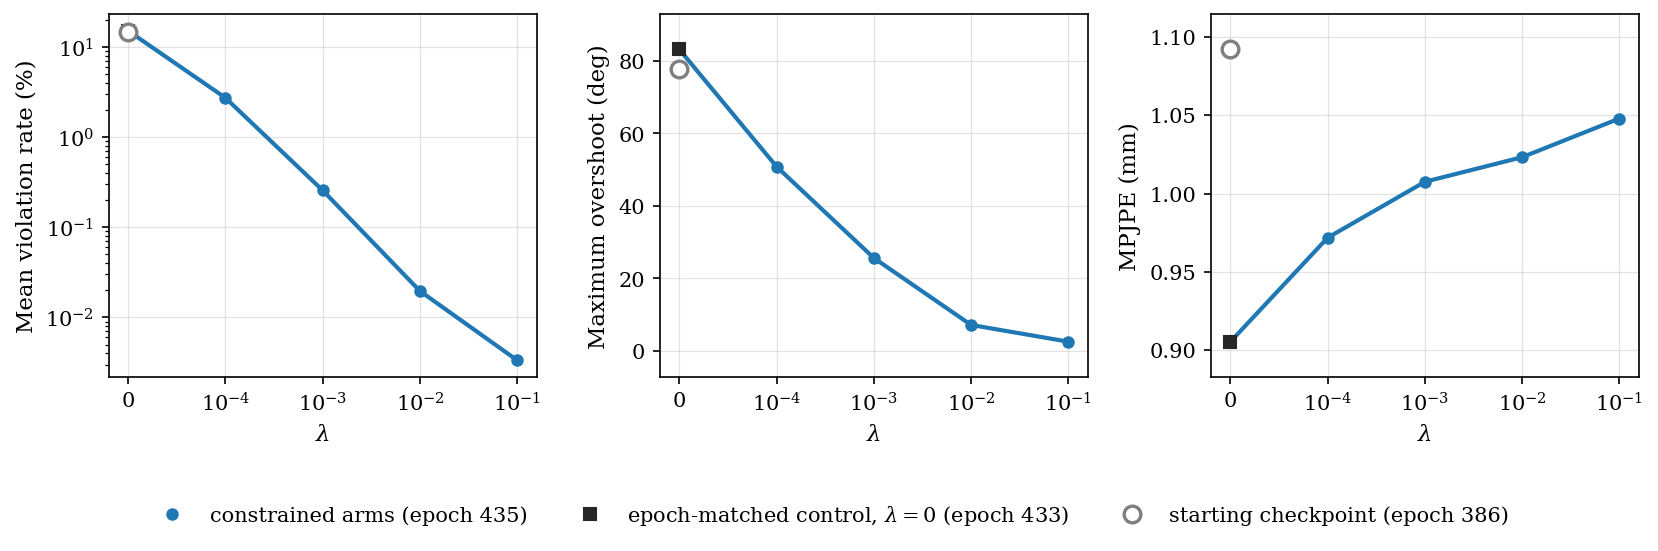
\includegraphics[width=\textwidth]{fig_tradeoff.pdf}
\caption{The plausibility/accuracy trade-off across four decades of $\lam$.
Violation rate is the mean fraction of frames outside the authored range over
the $162$ authored axes (log scale). Neither curve has an interior optimum:
plausibility improves and accuracy degrades with every decade from the
epoch-matched control (filled square, $\lam = 0$, epoch $433$). The open circle
is \armbase{} (epoch $386$): continued training without the prior improves
MPJPE but leaves plausibility where it was.}
\label{fig:tradeoff}
\end{figure}

\subsection{Anatomical plausibility}
\label{sec:res-plaus}

The prior is effective on the quantity it penalises (\Cref{tab:main},
\Cref{fig:tradeoff}). Relative to the epoch-matched control \armref{}, the mean
violation rate falls by a factor of $5.5$ at $\lam = 10^{-4}$, by $59$ at
$10^{-3}$, by $770$ at $10^{-2}$ and by $\approx\!4500$ at $10^{-1}$. Mean
overshoot on violating axes falls from \SI{2.78}{\degree} to below
\SI{0.001}{\degree}.

The control also shows that none of this comes from continued training. Over
the same $49$ epochs without the prior, plausibility does not improve and
slightly worsens: the mean violation rate goes from \SI{14.76}{\percent}
(\armbase{}) to \SI{15.11}{\percent}, and the maximum overshoot from
\SI{77.7}{\degree} to \SI{83.2}{\degree}. The whole plausibility gain in
\Cref{tab:main} is therefore due to the prior, just as the whole accuracy gain
over \armbase{} is due to continued training (\Cref{sec:res-acc}).

The number of axes violating \emph{at least once} is a poor summary: it falls
only from $94$ to $41$ while the rate falls by more than three orders of
magnitude, because it is a binary indicator over \num{50630} frames and a
single marginal frame is enough to trip it. The informative quantity is the
maximum overshoot, which measures how badly the worst predicted pose fails:
$83.2 \rightarrow 50.8 \rightarrow 25.6 \rightarrow 7.2 \rightarrow
\SI{2.5}{\degree}$. At $\lam = 10^{-4}$ the model still produces a
\SI{50.8}{\degree} violation somewhere in the test set --- rare, but
anatomically impossible. A requirement of the form ``no anatomically impossible
pose ever'' is met only from $\lam = 10^{-2}$ upwards.

\begin{figure}[t]
\centering
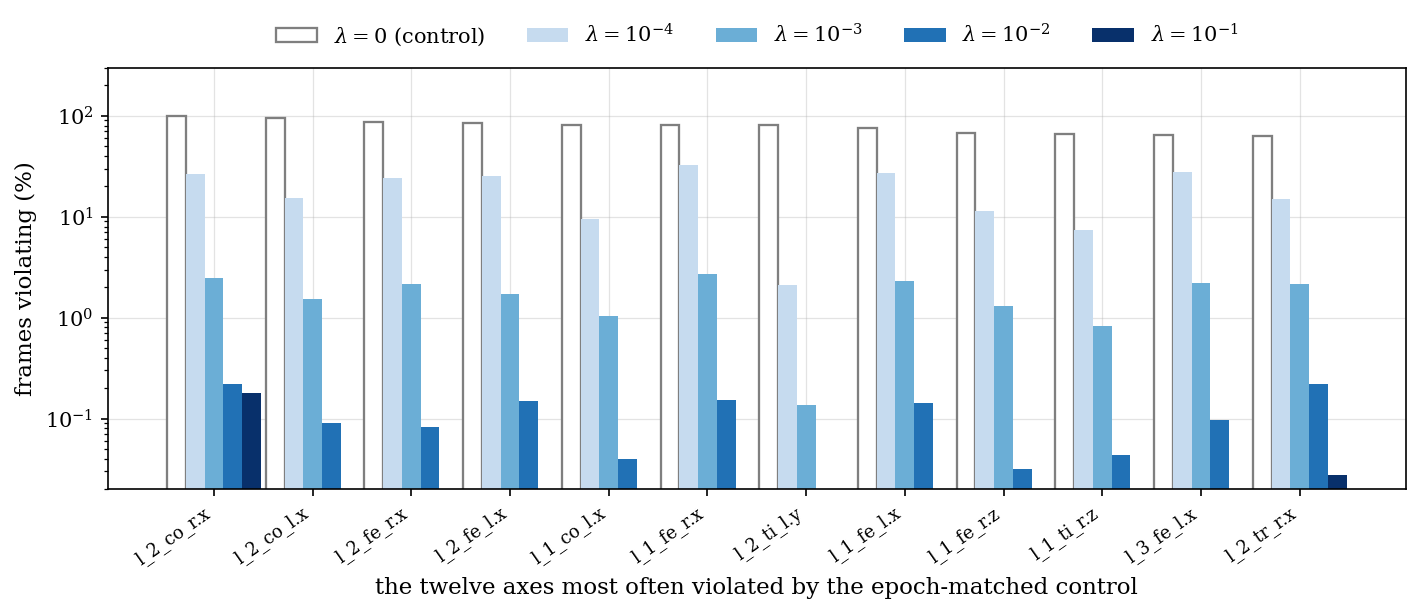
\includegraphics[width=0.92\textwidth]{fig_worst_axes.pdf}
\caption{The twelve axes most frequently violated by the epoch-matched control
\armref{}, and their violation rate under each $\lam$ (log scale; bars below
\SI{0.02}{\percent} are drawn at the axis floor). All twelve are leg axes,
predominantly coxa and femur. \armref{} violates \texttt{l\_2\_co\_r.x} on
\SI{98.9}{\percent} of frames; at $\lam = 10^{-1}$ the same axis violates on
\SI{0.18}{\percent}.}
\label{fig:worst}
\end{figure}

\Cref{fig:worst} shows where the violations are concentrated. All twelve of the
most-violated axes belong to the legs, and nine are femur or coxa axes
--- the degrees of freedom that dominate stance and swing. The prior therefore
acts, as intended, on anatomically meaningful joints rather than on numerically
incidental ones.

\subsection{Accuracy}
\label{sec:res-acc}

Compared with \armbase{}, the prior appears to be free: all four constrained
arms beat the starting checkpoint on MPJPE, median MPJPE, PCK and mean 2D
error. The epoch-matched control shows that this was entirely the effect of
continued training. \armref{} is the most accurate arm on every accuracy
metric in \Cref{tab:main}, and accuracy degrades monotonically with $\lam$
from $\lam = 0$ onward:
\begin{center}
\begin{tabular}{lccccc}
\toprule
 & $\lam=0$ & $10^{-4}$ & $10^{-3}$ & $10^{-2}$ & $10^{-1}$ \\
\midrule
MPJPE (mm)            & 0.9054 & 0.9718 & 1.0075 & 1.0232 & 1.0479 \\
\quad vs.\ \armref{}  & ---    & $+\SI{7.3}{\percent}$ & $+\SI{11.3}{\percent}$ & $+\SI{13.0}{\percent}$ & $+\SI{15.7}{\percent}$ \\
PCK@5\,px (native)    & 0.5110 & 0.4301 & 0.4024 & 0.3915 & 0.3745 \\
\quad vs.\ \armref{}  & ---    & $-\SI{15.8}{\percent}$ & $-\SI{21.3}{\percent}$ & $-\SI{23.4}{\percent}$ & $-\SI{26.7}{\percent}$ \\
Mean 2D error (px)    & 6.369  & 7.234  & 7.614  & 7.777  & 8.038  \\
\quad vs.\ \armref{}  & ---    & $+\SI{13.6}{\percent}$ & $+\SI{19.5}{\percent}$ & $+\SI{22.1}{\percent}$ & $+\SI{26.2}{\percent}$ \\
\bottomrule
\end{tabular}
\end{center}
Continued training alone improves on \armbase{} by \SI{17.1}{\percent} in
MPJPE ($1.0920 \rightarrow \SI{0.9054}{\milli\metre}$), by \SI{35.8}{\percent}
in native PCK@5\,px ($0.3762 \rightarrow 0.5110$) and by \SI{18.6}{\percent} in
mean 2D error. The prior consumes part of that gain: \SI{36}{\percent} of the
MPJPE gain at $\lam = 10^{-4}$ and \SI{76}{\percent} at $10^{-1}$. On native
PCK@5\,px it consumes \SI{60}{\percent} at $10^{-4}$ and all of it
(\SI{101}{\percent}) at $10^{-1}$.

A least-squares fit of MPJPE against $\log_{10}\lam$ over the four constrained
arms gives a slope of $\SI{0.0244}{\milli\metre}$ per decade ($R^2 = 0.98$),
i.e.\ \SI{2.7}{\percent} of \armref{} per decade. The cost is, however,
\emph{front-loaded}: the step from $\lam = 0$ to $10^{-4}$
(\SI{+0.066}{\milli\metre}) is worth $2.7$ decades of that slope. Switching the
prior on at all is the largest single cost in the sweep; strengthening it
afterwards is comparatively cheap.

\begin{figure}[t]
\centering
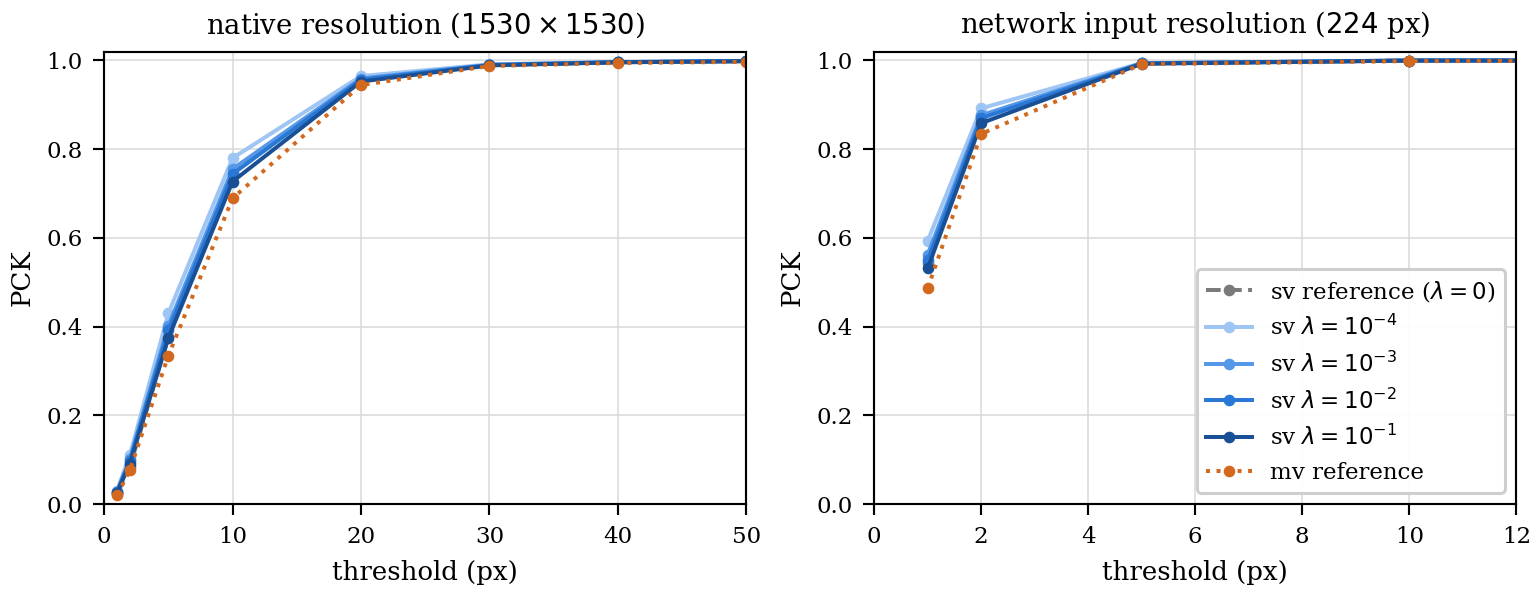
\includegraphics[width=\textwidth]{fig_pck.pdf}
\caption{PCK curves on the test split at both reporting resolutions. The four
constrained arms are ordered by $\lam$ at every threshold on both curves:
weaker regularisation is uniformly more accurate. The reference curve drawn is
\armbase{}; at the native resolution the $\lam = 10^{-1}$ curve falls below it
for thresholds of $5\,$px and above, despite $49$ additional epochs of
training. The epoch-matched \armref{} (native PCK@5\,px $0.5110$) is not yet
drawn.}
\label{fig:pck}
\end{figure}

This is not an artefact of a single threshold: in \Cref{fig:pck} the
constrained arms are ordered by $\lam$ at every point of both PCK curves, and
\armref{} lies above all of them at the $5\,$px threshold on both resolutions
($0.5110$ native, $0.9943$ at $224\,$px). The $\lam = 10^{-1}$ arm reaches
PCK@5\,px $=0.3745$ at native resolution against \armbase{}'s $0.3762$ ---
after $49$ additional epochs of training, it is \emph{worse} at placing
keypoints in the image than the checkpoint it started from, while the same
$49$ epochs at $\lam = 0$ raise that figure to $0.5110$.

\begin{figure}[t]
\centering
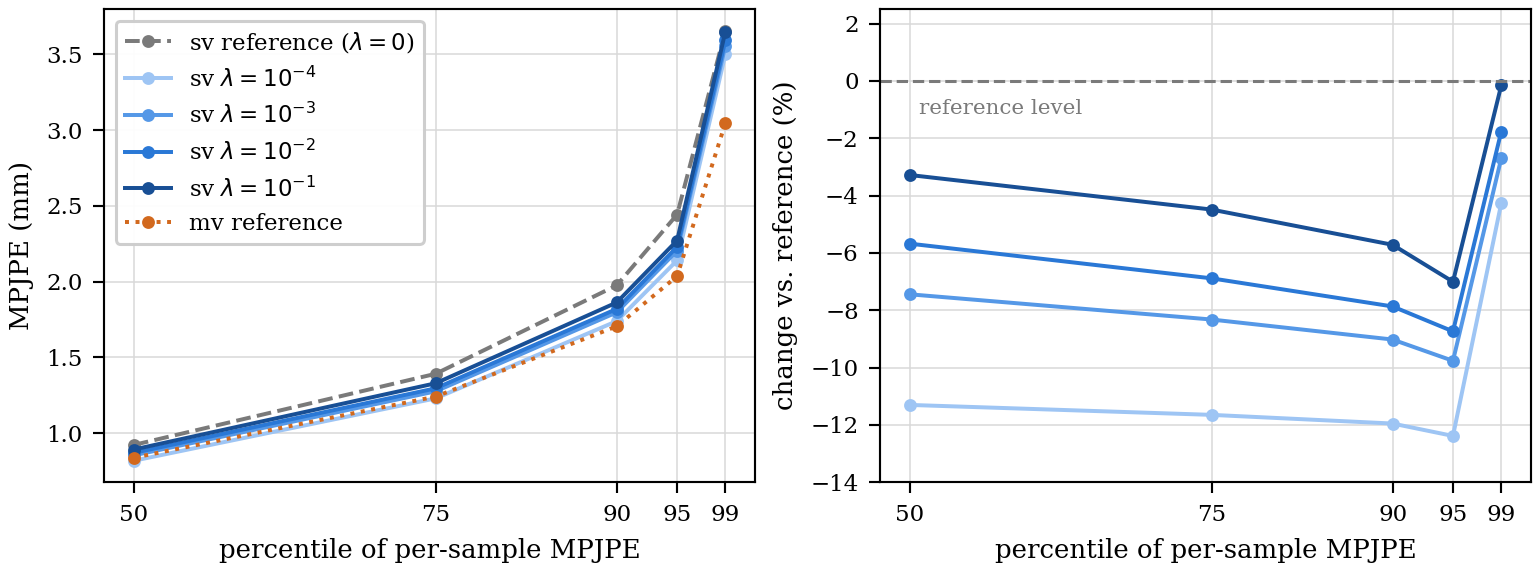
\includegraphics[width=\textwidth]{fig_mpjpe_quantiles.pdf}
\caption{Left: MPJPE quantile functions. Right: change relative to \armbase{}
at each percentile. The accuracy ordering is preserved across the whole error
distribution, and the gain of the constrained arms over \armbase{} shrinks
towards the tail (for $\lam = 10^{-4}$: $-\SI{11.3}{\percent}$ at P50 against
$-\SI{4.3}{\percent}$ at P99). Against the epoch-matched \armref{}
(P50 \SI{0.7439}{\milli\metre}, P99 \SI{3.3970}{\milli\metre}), the same arm
is $+\SI{10.0}{\percent}$ at P50.}
\label{fig:quant}
\end{figure}

\Cref{fig:quant} decomposes the 3D error by percentile. The ordering by $\lam$
holds across the entire error distribution, and the advantage of the
constrained arms over \armbase{} is largest at the median and smallest in the
tail. That is the signature of general fine-tuning: if the prior were the
cause of the improvement, the gain should concentrate in the tail, where the
implausible poses live. The epoch-matched control confirms this reading: at
the median, \armref{} is \SI{19.4}{\percent} better than \armbase{}, and every
constrained arm is worse than \armref{} (median MPJPE $+\SI{10.0}{\percent}$ at
$\lam = 10^{-4}$ to $+\SI{20.0}{\percent}$ at $10^{-1}$).

\subsection{Range of motion}
\label{sec:res-rom}

\begin{table}[t]
\centering
\small
\caption{Mean range of motion per bounded axis (deg), by joint group, over the
$129$ axes with a finite authored range. The clipping bound (\Cref{eq:clip}) is
the ROM the epoch-matched control \armref{} would retain if its trajectory were
merely clipped into the authored box. \armbase{} is given for comparison.}
\label{tab:rom}
\setlength{\tabcolsep}{4.5pt}
\begin{tabular}{l r r *{5}{r}}
\toprule
Joint group & axes & \armbase{} & $\lam{=}0$ & $10^{-4}$ & $10^{-3}$ & $10^{-2}$ & $10^{-1}$ \\
\midrule
Coxa            & 18 & 78.1 & 77.8 & 65.1 & 61.6 & 58.0 & 55.0 \\
Trochanter      & 18 & 74.2 & 71.9 & 52.1 & 44.7 & 39.1 & 36.9 \\
Femur           & 18 & 71.6 & 70.5 & 44.1 & 26.8 & 20.7 & 18.7 \\
Tibia           & 18 & 88.9 & 83.6 & 50.3 & 41.4 & 33.3 & 28.6 \\
Tarsus          & 18 & 96.3 & 92.0 & 54.1 & 48.2 & 43.0 & 38.0 \\
Antenna         & 18 & 40.9 & 40.2 & 33.7 & 31.8 & 30.6 & 30.0 \\
Head / wings    & 21 & 20.2 & 19.6 & 13.6 & 10.9 &  9.3 &  8.9 \\
\midrule
\textbf{All}    & \textbf{129} & \textbf{66.1} & \textbf{64.0} & \textbf{44.0} & \textbf{37.3} & \textbf{32.9} & \textbf{30.3} \\
\midrule
\multicolumn{3}{l}{\emph{Clipping bound} (of \armref{})} & \multicolumn{5}{c}{$36.3$ (mean over all $129$ axes)} \\
\multicolumn{3}{l}{\emph{Mean authored range}} & \multicolumn{5}{c}{$51.6$} \\
\bottomrule
\end{tabular}
\end{table}

Continued training without the prior barely changes the range of motion: the
mean ROM goes from \SI{66.1}{\degree} (\armbase{}) to \SI{64.0}{\degree}
(\armref{}), and no joint group changes by more than \SI{6}{\percent}
(\Cref{tab:rom}). The ROM changes below are therefore effects of the prior.

\armref{} moves through a mean ROM of \SI{64.0}{\degree} per bounded axis,
against a mean authored range of \SI{51.6}{\degree} --- a ratio of means of
$1.24\times$. Averaged per axis instead, the exceedance is larger, $1.89\times$
(\Cref{fig:ratio}), since axes with small authored ranges contribute
disproportionately large ratios; both figures describe the same overshoot from
different weightings and are not in conflict. Clipping the \armref{} trajectory
into the box would leave \SI{36.3}{\degree}. The constrained arms give $44.0$,
$37.3$, $32.9$ and \SI{30.3}{\degree} for $\lam = 10^{-4} \ldots 10^{-1}$
(\Cref{tab:rom}).

$\lam = 10^{-3}$ sits just above the clipping bound ($+\SI{2.7}{\percent}$).
From $\lam = 10^{-2}$ upward the model does not merely stay inside the authored
box --- it withdraws into the interior, ending $\SI{9.5}{\percent}$ below the
clipping bound at $10^{-2}$ and $\SI{16.5}{\percent}$ below it at $10^{-1}$.
Since \Cref{eq:penalty} has zero gradient there, this cannot be a direct
response to the penalty. The most plausible mechanism is that the network
cannot distinguish ``near the boundary'' from ``beyond it'' while its own
predictions carry noise, and so learns a safety margin: predicting
conservatively is the cheapest way to keep the expected hinge loss at zero.

\begin{figure}[t]
\centering
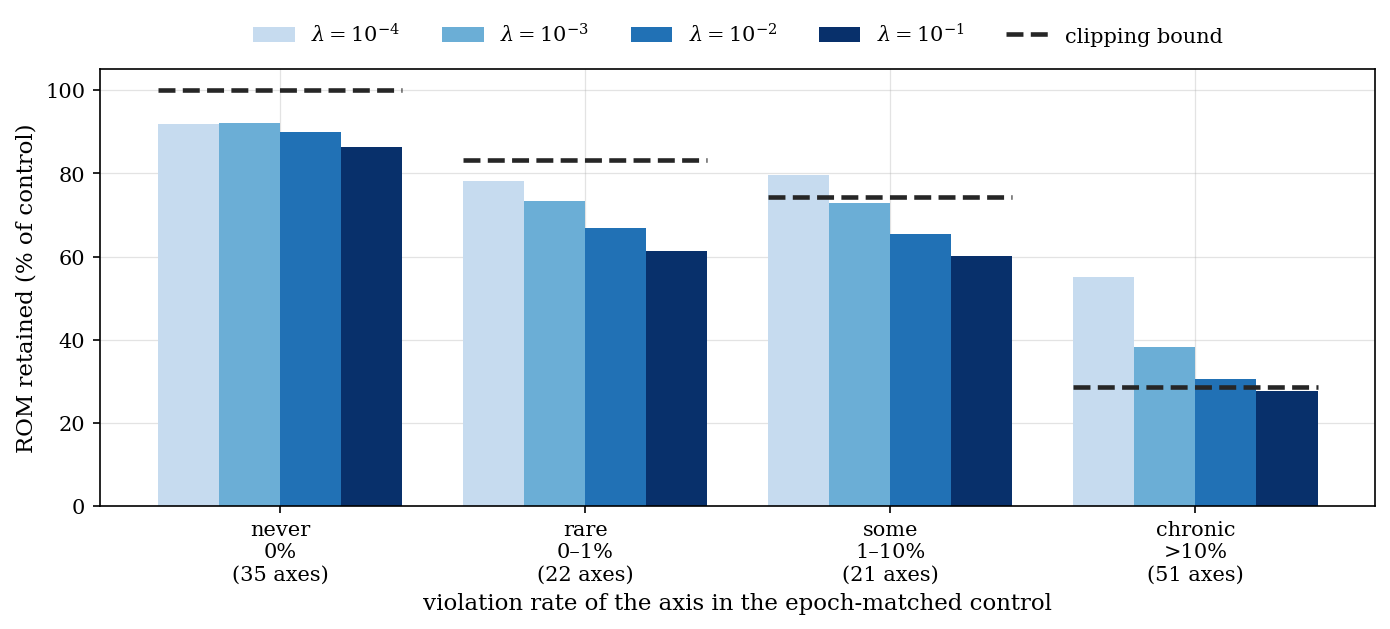
\includegraphics[width=0.86\textwidth]{fig_rom_retention.pdf}
\caption{ROM retained relative to the epoch-matched control \armref{}, with
axes grouped by \armref{}'s own violation rate on that axis (retention pooled
over the axes of each group). The dashed rule in each group is the clipping
bound of \Cref{eq:clip} --- the retention that pure violation removal would
produce. Axes that never violated retain \SIrange{86.4}{92.1}{\percent} of
their range. On chronically violating axes $\lam = 10^{-2}$ sits just above
the clipping bound (\SI{30.5}{\percent} vs.\ \SI{28.7}{\percent}) and
$\lam = 10^{-1}$ just below it (\SI{27.7}{\percent}).}
\label{fig:retention}
\end{figure}

\Cref{fig:retention} resolves the effect by axis severity, with two results of
opposite sign. The prior is \emph{mostly targeted}: the $35$ axes that never
violated in \armref{} retain \SIrange{86.4}{92.1}{\percent} of their range,
far more than the violating axes do, although they still lose
\SIrange{8}{14}{\percent} and the loss grows at $\lam = 10^{-1}$. But it
\emph{overshoots on marginal axes}: on axes that violated on less than
\SI{1}{\percent} of frames, $\lam = 10^{-1}$ retains only \SI{61.3}{\percent}
of the \armref{} range where clipping would retain \SI{83.2}{\percent} ---
$22$ percentage points of motion removed for which no violation can account.

\begin{figure}[t]
\centering
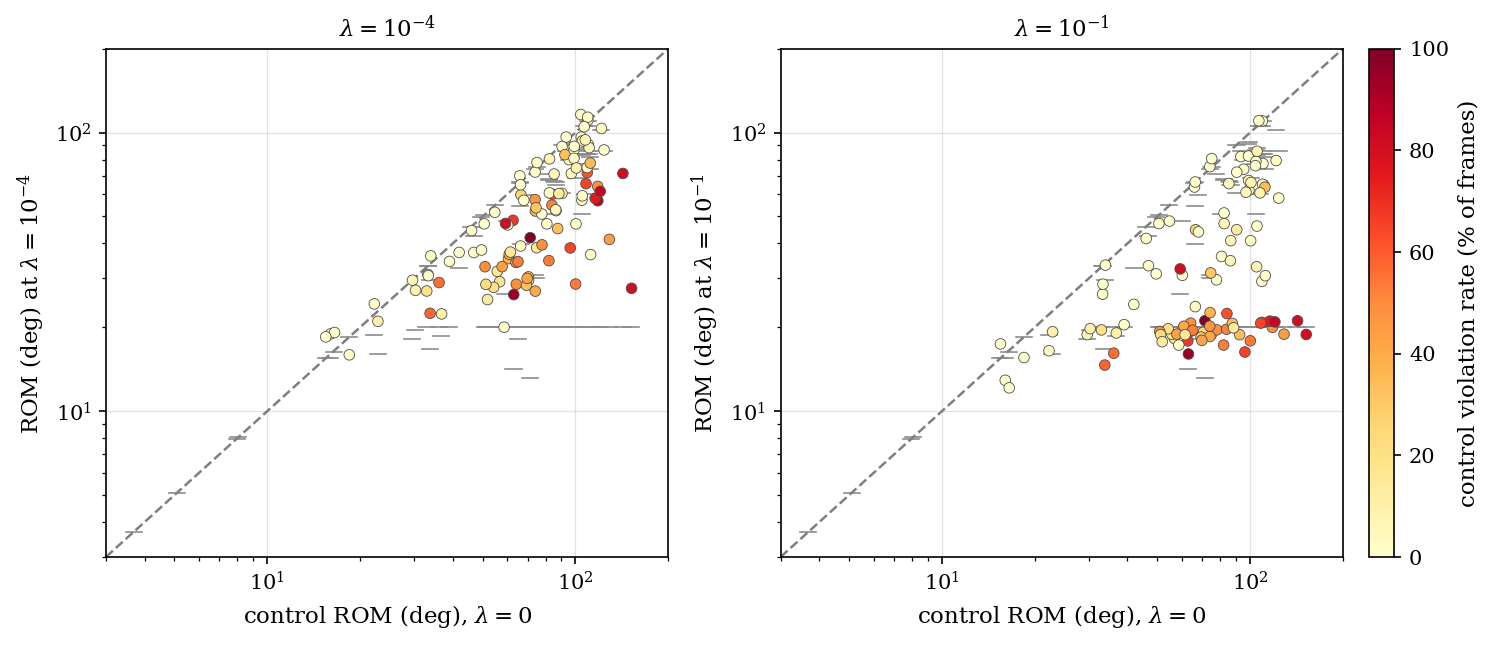
\includegraphics[width=\textwidth]{fig_rom_scatter.pdf}
\caption{Per-axis ROM of \armref{} against the constrained arms (log--log).
Marker colour encodes the \armref{} violation rate; horizontal ticks mark the
clipping bound for each axis. At $\lam = 10^{-4}$ most axes sit near or above
their clipping bound. At $\lam = 10^{-1}$ a dense band of axes has collapsed to
roughly \SIrange{15}{25}{\degree} regardless of its starting ROM, which is the
visual signature of the learned margin.}
\label{fig:scatter}
\end{figure}

\begin{figure}[t]
\centering
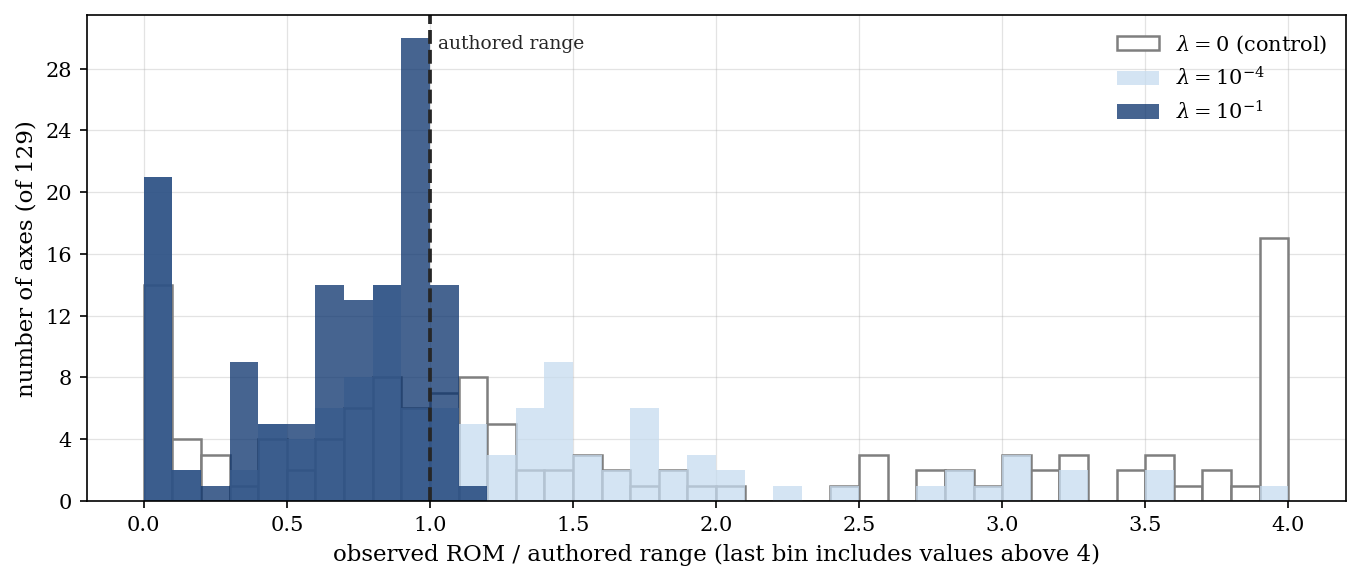
\includegraphics[width=0.86\textwidth]{fig_rom_ratio.pdf}
\caption{Distribution over the $129$ bounded axes of the ratio between observed
ROM and authored range (ratios above $4$ are collected in the last bin).
\armref{} (mean $1.89$, median $1.19$; $77$ axes above $1.0$) systematically
exceeds the authored envelope. By $\lam = 10^{-1}$ only $15$ axes reach it and
the mean ratio is $0.66$, i.e.\ the typical joint uses barely two-thirds of the
range it is permitted.}
\label{fig:ratio}
\end{figure}

\Cref{fig:scatter,fig:ratio} display the same phenomenon per axis and in
distribution. \Cref{tab:rom} shows where it is paid for: relative to \armref{},
femur ROM falls from \SI{70.5}{\degree} to \SI{18.7}{\degree}
($-\SI{73}{\percent}$), tibia from \SI{83.6}{\degree} to \SI{28.6}{\degree}
($-\SI{66}{\percent}$) and tarsus by \SI{59}{\percent}, while coxa loses only
\SI{29}{\percent} and antennae \SI{25}{\percent}. The femur--tibia complex is
the principal locomotor degree of freedom of the stick insect; a model whose
femora sweep through less than \SI{19}{\degree} will render a visibly stiff
gait irrespective of its MPJPE.

\subsection{Spread versus centre}
\label{sec:res-centre}

The original analysis measured the mean absolute shift of the per-axis mean
angle relative to \armbase{}: $4.20$, $4.38$, $4.50$ and \SI{4.69}{\degree} for
$\lam = 10^{-4} \ldots 10^{-1}$. Because this was nearly constant across four
decades, it was attributed to the $49$ epochs of continued training. The
epoch-matched control rules that out. \armref{} moves the centre by only
\SI{1.79}{\degree} relative to \armbase{}, and relative to \armref{} the
constrained arms are shifted by $4.48$, $4.68$, $4.79$ and \SI{4.96}{\degree}.

The centre shift is therefore caused by the prior, and almost all of it
appears as soon as the prior is switched on; strengthening the prior by three
decades adds only \SI{11}{\percent}. This mirrors the accuracy result of
\Cref{sec:res-acc}, where most of the MPJPE cost is paid at $\lam = 10^{-4}$.
The prior thus acts in two ways: a step change in the centre of the pose
distribution that appears at switch-on, and a graded contraction of its spread
that grows with $\lam$ (\Cref{sec:res-rom}). A plausible link between the two
is that the switch-on shift moves typical poses away from the data, which
would account for the step in accuracy cost, but this has not been tested
directly.

%==============================================================================
\section{Discussion}
\label{sec:discussion}

\subsection{The fine-tuning confound}
\label{sec:disc-confound}

In the original design every ``constrained beats reference'' comparison
contrasted \emph{prior plus $49$ epochs} against \emph{neither}: the correct
control --- $\lam = 0$ continued for the same epochs --- was missing. Three
observations indicated that the accuracy gain belonged to the fine-tune rather
than the prior: (i) within the constrained arms every accuracy metric degrades
monotonically with $\lam$; (ii) linear extrapolation of MPJPE in
$\log_{10}\lam$ placed a hypothetical $\lam = 10^{-5}$ arm at
$\approx\SI{0.95}{\milli\metre}$, below every constrained arm; (iii) the
$\lam = 10^{-1}$ arm already fell below \armbase{} on native PCK@5\,px despite
$49$ additional epochs.

The control has now been run, and it confirms all three. \armref{} reaches
\SI{0.9054}{\milli\metre} MPJPE --- lower even than the extrapolated
$\lam = 10^{-5}$ estimate --- and is the most accurate arm on every metric in
\Cref{tab:main}. The whole of the apparent improvement over \armbase{} is due
to continued training (\SI{-17.1}{\percent} MPJPE at $\lam = 0$), and the prior
subtracts from it at every $\lam$ (\Cref{sec:res-acc}). That the measured value
lies below the extrapolation is itself informative: the cost of the prior is
not linear in $\log_{10}\lam$ all the way down, but has a step at switch-on.

The control settles plausibility in the same way. Over the same $49$ epochs
without the prior, the violation rate does not improve
(\Cref{sec:res-plaus}), and the range of motion and the centre of the pose
distribution barely move (\Cref{sec:res-rom,sec:res-centre}). The
plausibility gain and the ROM loss are therefore effects of the prior, and the
accuracy gain over \armbase{} is an effect of training alone.

What can now be stated is: \emph{the prior buys a large plausibility gain at a
measured accuracy cost of $+\SI{7.3}{\percent}$ to $+\SI{15.7}{\percent}$
MPJPE and $-\SI{15.8}{\percent}$ to $-\SI{26.7}{\percent}$ native PCK@5\,px
over the four decades tested.}

\subsection{Over-regularisation and the learned margin}

The ROM analysis identifies a failure mode that the violation rate cannot see.
A one-sided hinge is, by construction, inactive inside the feasible set; yet
for $\lam \ge 10^{-2}$ the model settles well inside it (\Cref{sec:res-rom}).
Two mechanisms are consistent with the evidence and are not mutually exclusive:
(a) prediction noise makes a near-boundary configuration risky in expectation,
so the minimum-risk prediction sits at a margin; (b) the penalty is applied to
a batch mean, so a systematic inward bias across many axes is a cheap way to
reduce it. Distinguishing them, and mitigating the effect, is the object of the
tolerance-band and annealing experiments proposed in \Cref{sec:next}.

\subsection{Limitations of the plausibility metric}

The violation rate is minimised by a stiff pose, and \Cref{sec:res-rom} shows
the sweep exploiting exactly that degree of freedom, so a plausibility claim
resting on the violation rate alone is not sound. It should be paired with an
under-articulation measure --- the per-axis ratio of observed ROM to authored
range (\Cref{fig:ratio}) is the natural candidate --- so that a model cannot
score as plausible by ceasing to move.

\subsection{Choice of operating point}

The clipping-bound analysis (\Cref{fig:retention}) favours $\lam = 10^{-2}$: it
is the strongest setting at which chronically violating axes still sit above
the bound (\SI{30.5}{\percent} vs.\ \SI{28.7}{\percent}), while violations are
effectively eliminated
(max.\ overshoot \SI{7.2}{\degree}) at an MPJPE cost of
\SI{0.118}{\milli\metre} ($+\SI{13.0}{\percent}$) and a native PCK@5\,px cost
of $-\SI{23.4}{\percent}$ relative to the epoch-matched \armref{}. We recommend
it as the default when plausibility is an explicit requirement, since
$\lam = 10^{-4}$ still admits \SI{50.8}{\degree} overshoots.

Where 3D accuracy is the priority, $\lam = 10^{-3}$ is the better compromise:
violation rate \SI{0.26}{\percent}, MPJPE \SI{1.0075}{\milli\metre}
($+\SI{11.3}{\percent}$), and a mean ROM just above the clipping bound
(\SI{37.3}{\degree} vs.\ \SI{36.3}{\degree}).
Because most of the cost is paid at switch-on, the difference between
$10^{-3}$ and $10^{-2}$ is small (\SI{0.016}{\milli\metre}); if plausibility is
not required at all, the unregularised \armref{} is the most accurate
single-view model measured. $\lam = 10^{-1}$ is not recommended at any
operating point: its marginal plausibility gain over $10^{-2}$ is small
(\SI{7.2}{\degree} to \SI{2.5}{\degree} of maximum overshoot) and it costs
\SI{73}{\percent} of femur range, $+\SI{15.7}{\percent}$ MPJPE and
$+\SI{26.2}{\percent}$ mean 2D error relative to \armref{}.

\subsection{Threats to validity}

Three caveats bound the conclusions. First, two figures
(\Cref{fig:pck,fig:quant}) still draw \armbase{} rather than \armref{} as the
reference, because the benchmark reports of the constrained arms are not in
the repository; the numbers quoted against \armref{} in the text are taken
from its evaluation log. Second, \armref{} is scored at the
validation-best epoch $433$, whereas the constrained arms are scored at the
fixed epoch $435$; selection on validation loss gives \armref{} a small
advantage that is unlikely to account for a gap of \SI{0.066}{\milli\metre} or
more, but the arms are not selected identically. Third, ROM as defined here is a min--max statistic
over the test set and is therefore sensitive to outliers; the distributional
view in \Cref{fig:ratio} and the per-axis view in \Cref{fig:scatter} are
provided so that the aggregate is not read in isolation.

%==============================================================================
\section{Conclusion}
\label{sec:conclusion}

Returning to the question of \Cref{sec:intro}:

\begin{description}[leftmargin=1.4em,style=nextline]
\item[More anatomically plausible poses --- yes.]
  Across four decades the authored prior reduces the mean violation rate by
  between $5.5\times$ and $4500\times$ relative to the epoch-matched control,
  and the worst overshoot from \SI{83.2}{\degree} to \SI{2.5}{\degree}, acting
  on precisely the leg axes that dominate locomotion. Continued training
  without the prior produces none of this gain.
\item[Without losing accuracy --- no.]
  The apparent gain over the starting checkpoint came from $49$ epochs of
  continued training. Against the epoch-matched $\lam = 0$ control, every
  constrained arm is less accurate: $+\SI{7.3}{\percent}$ to
  $+\SI{15.7}{\percent}$ MPJPE and $-\SI{15.8}{\percent}$ to
  $-\SI{26.7}{\percent}$ native PCK@5\,px, with most of the cost incurred as
  soon as the prior is switched on.
\end{description}

A third finding was not anticipated by the study design: the prior does more
than remove violations. From $\lam = 10^{-2}$ it induces a conservative
inward bias that costs the femur and tibia most of their range of motion, in a
region where the penalty exerts no gradient at all. Plausibility, in the sense
that matters for behavioural analysis, is not only a matter of staying inside
the authored box but also of using it.

%==============================================================================
\section{Next step}
\label{sec:next}

\begin{enumerate}[leftmargin=1.9em,itemsep=0.45em]

\item Copy the benchmark reports of the single-view constrained arms into
      the repository and redraw \Cref{fig:pck,fig:quant} against \armref{}.
\item Given the step cost at switch-on, test weaker settings
      ($10^{-6}$, $10^{-5}$) to see whether any part of the plausibility gain
      can be had at a smaller accuracy cost.
\item Sweep additional magnitudes of $\lam$: $5{\times}10^{-2}$,
      $5{\times}10^{-1}$, $1$, $5$, $10$.
\item Apply the same pipeline to the multi-view case: find a solution for the compute wall.
\end{enumerate}

%==============================================================================
\appendix
\sloppy
\section{Data provenance}
\label{app:prov}

\begin{description}[leftmargin=0em,style=nextline,itemsep=0.25em,font=\normalfont\ttfamily\small]
\item[prior\_study\_results/sweep/\{sweep.csv, arms.csv, comparison.md\}]
  Aggregated sweep metrics; source of the violation and MPJPE columns of
  \Cref{tab:main}.
\item[prior\_study\_results/\{sv\_reference,
  lam1e-\{1..4\}/sv\_constrained\}/analysis/]
  Per-arm \texttt{limit\_violations.csv}, \texttt{per\_axis\_stats.csv} and
  \texttt{magnitude\_stats.csv} for \armbase{} and the constrained arms.
\item[prior\_study\_results\_matched/sv\_reference/analysis/]
  The same files for the epoch-matched control \armref{}; together with the
  above, source of the plausibility columns of \Cref{tab:main} and of all ROM,
  retention and centre-shift analyses.
\item[benchmark\_*\_on\_SMILySTICKS\_centred\_reprojected\_FIXED/benchmark\_report.txt]
  Per-arm PCK curves, 2D errors and MPJPE percentiles;
  source of \Cref{fig:pck,fig:quant}.
\item[logs/jl\_train\_3961264\_8.out, logs/jl\_eval\_4097171\_10.out]
  Training and evaluation of the epoch-matched control \armref{}; source of
  its row in \Cref{tab:main} and of all accuracy deltas against it.
\item[3D\_model\_prep/SMILy\_STICK\_limits\_authored.pkl]
  Authored per-joint rotation limits (\texttt{joint\_limits}), against which all
  arms are scored.
\item[report\_joint\_limit\_prior/make\_matched\_figures.py]
  Script regenerating \Cref{fig:tradeoff,fig:worst,fig:retention,fig:scatter,fig:ratio}
  against \armref{} from the sources above. \Cref{fig:pck,fig:quant} come from
  the original \texttt{make\_figures.py}.
\end{description}

\noindent
The clipping bound (\Cref{eq:clip}), the ROM retention buckets
(\Cref{fig:retention}) and the joint-group aggregation (\Cref{tab:rom}) are
derived in this report and are not present in the original sweep outputs.

\end{document}
